\section{Terrains}

Cette section permet à l'utilisateur, propriétaires d'un terrain, de gérer ses terrains : il peut ajouter, modifier, et supprimer des terrains qui lui impartient pour Le Charles de Lorraine.

\subsection{Ajouter un terrain}

Pour ajouter un terrain, il faut accéder à la page "Terrains" du menu de navigation en dessous du logo du site web. Sur cette page, il est possible d'ajouter un terrain en cliquant sur le bouton "Enregistrer un nouveau terrain" en bas de la page.

\begin{figure}[H]
\centering
\includegraphics[scale=0.15]{user_images/basic_user/GererTerrains/AjoutTerrain/001.jpg}
\caption{Ajouter un terrain, étape 1}
\end{figure}

Sur cette page, un formulaire d'informations sur le nouveau terrain vous est demandé. Il est décomposé en 2 parties : la première concerne le terrain à tout moment, et la deuxième concerne uniquement pour cette année-ci.

\begin{figure}[H]
\centering
\includegraphics[scale=0.15]{user_images/basic_user/GererTerrains/AjoutTerrain/002.jpg}
\caption{Ajouter un terrain, étape 2}
\end{figure}

Dès vous avez rempli le formulaire, vous pouvez finaliser l'enregistrement du terrain en cliquant sur le bouton "Ajouter" en bas de la page.

\begin{figure}[H]
\centering
\includegraphics[scale=0.15]{user_images/basic_user/GererTerrains/AjoutTerrain/003.jpg}
\caption{Ajouter un terrain, étape 3}
\end{figure}

La page des terrains est mise à jour, avec le nouveau terrain ajouté. À droite, une liste précise les activités liés à tous les terrains de l'utilisateur : si un terrain est choisi pour un tournoi, cette information sera automatiquement communiquée à cet utilisateur. 

\begin{figure}[H]
\centering
\includegraphics[scale=0.15]{user_images/basic_user/GererTerrains/AjoutTerrain/004.jpg}
\caption{Ajouter un terrain, étape 4}
\end{figure}

\subsection{Modifier un terrain}

Pour modifier les informations d'un terrain, l'utilisateur doit cliquer sur le terrain qu'il souhaite modifier, dans la liste "Mes terrains".

\begin{figure}[H]
\centering
\includegraphics[scale=0.15]{user_images/basic_user/GererTerrains/EditerTerrain/001.jpg}
\caption{Modifier un terrain, étape 1}
\end{figure}

Ensuite, l'utilisateur doit modifier le formulaire, similaire qu'au moment de la création du terrain, à la différence près qu'il est déjà pré-rempli avec les informations courantes.

\begin{figure}[H]
\centering
\includegraphics[scale=0.15]{user_images/basic_user/GererTerrains/EditerTerrain/002.jpg}
\caption{Modifier un terrain, étape 2}
\end{figure}

Dès que les modifications des chanps souhaités sont entrées, cliquez sur "Editer" en bas de la page pour confirmer les modifications des informations du tournoi.

\begin{figure}[H]
\centering
\includegraphics[scale=0.15]{user_images/basic_user/GererTerrains/EditerTerrain/003.jpg}
\caption{Modifier un terrain, étape 3}
\end{figure}

Vous pourrez voir, sur la page de vos terrains, que le terrain en question a bien été modifié.

\begin{figure}[H]
\centering
\includegraphics[scale=0.15]{user_images/basic_user/GererTerrains/EditerTerrain/004.jpg}
\caption{Modifier un terrain, étape 4}
\end{figure}

\subsection{Supprimer un terrain}

Pour supprimer un terrain, vous devez cliquer sur le terrain souhaité dans la liste de vos terrains.

\begin{figure}[H]
\centering
\includegraphics[scale=0.15]{user_images/basic_user/GererTerrains/SupprimerTerrain/001.jpg}
\caption{Supprimer un terrain, étape 1}
\end{figure}

Ensuite, vous devez cliquer sur le bouton "Supprimer" en bas de la page.

\begin{figure}[H]
\centering
\includegraphics[scale=0.15]{user_images/basic_user/GererTerrains/SupprimerTerrain/002.jpg}
\caption{Supprimer un terrain, étape 2}
\end{figure}

Une boîte de dialogue vous demande de confirmer la demande de suppression du terrain, puisque cette action est irréversible.

\begin{figure}[H]
\centering
\includegraphics[scale=0.15]{user_images/basic_user/GererTerrains/SupprimerTerrain/003.jpg}
\caption{Supprimer un terrain, étape 3}
\end{figure}

Après avoir validée l'action, votre terrain sera bien supprimé.

\begin{figure}[H]
\centering
\includegraphics[scale=0.15]{user_images/basic_user/GererTerrains/SupprimerTerrain/004.jpg}
\caption{Supprimer un terrain, étape 4}
\end{figure}
